\chapter{Fundamentos metodol\'ogicos}

	Se plante\'o la estructura a seguir por el trabajo, detallando el enfoque, tipo, nivel, dise\~no de la investigaci\'on y la metodolog\'ia implementada entre otros, el cual fue de vital importancia para el desarrollo de la misma. 
	
\section{Enfoque de la investigaci\'on}
	
	La investigaci\'on se desarrollo siguiendo un enfoque cuantitativo, como lo indican  \citet{pallela}, “la investigaci\'on cuantitativa requiere el uso de instrumentos de medici\'on y comparaci\'on, proporcionando datos cuyo estudio necesita la aplicaci\'on de m\'odelos matem\'aticos y estad\'isticos, el conocimiento est\'a basado en hechos”.  

\section{Tipo o nivel de investigaci\'on}
	
	Este proyecto plante\'o un tipo de investigaci\'on de campo, seg\'un como lo indican \citet{pallela},  la investigaci\'on de campo “consiste en la recolecci\'on directamente de la realidad donde ocurren los hechos, sin manipular o controlar variables” ya que permite indagar los efectos de la interrelaci\'on entre los diferentes tipos de variable en lugar de los hechos.\\

	En este punto se debe determinar la profundidad que abarca esta investigaci\'on, teniendo en cuenta que de acuerdo con \citet{arias} el nivel de la investigaci\'on es definido como “grado de profundidad con que se aborda un fen\'omeno u objeto de estudio”\\

	En este sentido, se tiene que dadas las caracter\'isticas del proyecto, se asocia con un nivel descriptivo, tal como lo indican \citet{pallela},  “hace \'enfasis sobre conclusiones dominantes o sobre como una persona, grupo o cosa se conduce o funciona en el presente” esto debido a que se medir\'an los datos extra\'idos sin alterarlos para ser mostrados en el sistema.\\

	Cuando se habla de un nivel descriptivo junto con una investigaci\'on de tipo de campo, en ella no se formulan hip\'otesis y las variables se enuncian en los objetivos de la investigaci\'on desarrollada.
	
\section{Dise\~no de investigaci\'on}
	
	Seg\'un \citet{arias}, el dise\~no de la investigaci\'on es “la estrategia general que adopta el investigador para responder al problema planteado”  puesto es vital establecer una correcta secuencia de pasos para elaborar el prototipo de  \textit{software}  dando soluci\'on a la problem\'atica principal de la investigaci\'on. \\
	
	Con este enfoque, es evidente entonces, el trabajo segui\'o un dise\~no no experimental para datos longitudinales retrospectivos, enfocado en el uso de informaci\'on existente, de acuerdo con lo dicho por  \citet{pallela} al definir el dise\~no no experimental como:

\begin{quote}
Es el que se realiza sin manipular en forma deliberada ninguna variable. El investigador no sustituye intencionalmente las variables independientes. Se observan los hechos tal y como se presentan en su contexto real y en un tiempo determinado o no, para luego analizarlos. Por lo tanto, este dise\~no no se construye una situaci\'on espec\'ifica sino que se observan las que existen. Las variables independientes ya han ocurrido y no pueden ser manipuladas, lo que impide influir sobre ellas para modificarlas. 
\end{quote}

	Esto indica que no hubo manipulaci\'on de variables. Esta investigaci\'on presenta una modalidad de proyecto especial que, como lo indican \citet{pallela}, los proyectos especiales “destinados a la creaci\'on de productos que puedan solucionar deficiencias evidenciadas, se caracterizan por su valor innovador y aporte significativo”, ya que se crear\'a un \textit{software} aplicable al \'area de estudio.

\section{Poblaci\'on y muestra}

Seg\'un \citet{morles} la poblaci\'on o universo al conjunto para el cual fueron validas las conclusiones que se obtuvieron de los elementos o las unidades (personas, instituciones o cosas) involucradas en la investigaci\'on.\\

En este sentido, se tiene que para las fases de elaboraci\'on y pruebas del prototipo de \textit{software}, se plante\'o utilizar archivos con extesi\'on .csv, como formato de datos de entrada a la aplicaci\'on.\\

La informaci\'on para los archivos de prueba proviene de vistas minables de la base de datos de tipo relacional, desarrollada en \textit{PostgreSQL} del Laboratorio de Investigaciones Hormonales del Instituto Aut\'onomo Hospital Universitario de los Andes, que alberga al programa para pacientes con VIH, que cuenta con una poblaci\'on registrada de 45.649\\

Esta informaci\'on fue  filtrada, par considerando los siguientes criterios:\\
\begin{itemize}
    \item La base de datos del Laboratorio de Investigaciones Hormonales IAHULA, no s\'olo almacena informaci\'on del Programa de Pacientes con VIH, las vistas minables estan conformadas por pacientes confirmados por las pruebas \textit{Elisa} y {Western Blot} para VIH
    \item En las vistas minables para  las pruebas s\'olo se categorizar\'an pacientes con residencia en el Estado Mérida
    \item Las vistas minables s\'olo las integraran pacientes con m\'as de tres años en seguimiento. Dado que los modelos son para datos longitudinales.
    \item Se categorizaron los pacientes por semestres y en cada lapso en medicados y no medicados.
\end{itemize}

Bajo estas condiciones se generó una vista minable (muestra) con 115 registros de pacientes, con una secci\'on transversal conformada por la edad el g\'enero y el municipio de residencia  y una secci\'on longitudinal con  informaci\'on entre Enero del año 2007 y Diciembre del año 2013. sobre el Log$_{10}$ de la carga viral plasm\'atica y las sub-poblaciones linfocitaria de c\'elulas T$^{+}$ CD4 y  T$^{+}$ CD8.\\

\section{T\'ecnicas e instrumentaci\'on para la recolecci\'on de datos}

En el desarrollo de este prototipo de \textit{software} es de vital importancia contar con una correcta t\'ecnica de recolecci\'on de datos y un instrumento adecuado para dicha t\'ecnica, pues fueron la base para lograr un efectivo an\'alisis estad\'istico, y as\'i como eficaces resultados en la fase de pruebas. Todo esto, teniendo en cuenta que, seg\'un \citet{hurtado} la selecci\'on de t\'ecnicas e instrumentos de recolecci\'on de datos implica determinar por cu\'ales medios o procedimientos el investigador obtendr\'a la informaci\'on necesaria para alcanzar los objetivos de la investigaci\'on.\\

Para efectos de esta investigaci\'on, se tuv\'o que la t\'ecnica de recolecci\'on de datos seleccionada es la observaci\'on no participante, indirecta y estructurada, la cual se ajusta a este de investigaci\'on, ya que como lo indican \citet{pallela} la observaci\'on es indirecta:

\begin{quote}
Cuando el investigador entra en conocimiento del hecho o fen\'omeno a trav\'es de las observaciones realizadas anteriormente por otra persona. Esto \'ultimo ocurre cuando se utilizan libros, revistas, informes, grabaciones, fotograf\'ias, realizadas con lo que se esta investigando, los cuales han sido obtenidos o elaborados por personas que antes se ocuparon de lo mismo.
\end{quote}

Esto debido, a que los datos usados provienen de la data existente del IAHULA, las cuales fueron tomadas previamente por otro investigador, por lo que no se intervino directamente en su recolecci\'on. Para esta fase de la investigaci\'on se realiz\'on una exportaci\'on de las tablas que conforman la base de datos que almacenaban informaci\'on sobre: Paciente, Pruebas, Resultados a archivos de texto plano, luego estos archivos fueron exportados a \textit{Microsoft Oficce Excel}, con formato .cvs donde los registros por pacientes fueron filtrados para conformar muestras an\'onimas y su direcci\'on categorizarla por municipios.
\section{Entorno de trabajo}

\subsection{\textit{Software} de desarrollo}

Para la realizaci\'on del prototipo de \textit{software}, fue necesario definir el entorno de desarrollo usado, se selecciono el lenguaje de programaci\'on R, dado que es un lenguaje de c\'odigo abierto bajo el paradigma de desarrollo colaborativo.  Como  herramienta de desarrollo integrada \textit{Integrated Development Environment, IDE} para lenguaje  R, se seleccion\'o  RStudio, dado su bran abanico de paquetes e integraci\'on con repositorios Git  que permite llevar  un control de versiones del sistema apoyado en el servicio de alojamiento gratuito de GitHub.

\subsection{\textit{Hardware} utilizado}

En la parte de hardware usado, se cuent\'o con dos computadoras (laptop y de PC de escritorio), con las caracter\'isticas descritas en la tabla:

\begin{table}[H]
\begin{center}
\begin{tabular}{|l|l|l|l|}
\hline
Componente & Laptop & PC Escritorio \\ \hline
CPU & Intel Core i3-380 & Intel Core i5-2310 \\ \hline
RAM & 4GB & 4GB \\ \hline
S.O & Windows 7 Ultimate & Windows 10  \\ \hline

\end{tabular}
\caption{Caracter\'isticas de los computadores a usar}
\label{tabla:componente}
\end{center}
\end{table}

\section{Metodolog\'ia}

Para el desarrollo de este trabajo se implement\'o  una metodolog\'ia para el desarrollo del \textit{software} en espiral  la es un m\'odelo del ciclo de vida del \textit{software} donde el esfuerzo del desarrollo es iterativo, tan pronto termina un esfuerzo, ah\'i mismo comienza el otro; adem\'as en cada ejecuci\'on del desarrollo se sigue cuatro pasos principales:

1. Determinar o fijar los objetivos: se definen los objetivos espec\'ificos para posteriormente identificar las limitaciones del proceso y del sistema de \textit{software}; adem\'as se dise\~na una planificaci\'on detallada de gesti\'on y se identifican los riesgos.

2. An\'alisis de riesgo: se efect\'ua un an\'alisis detallado para cada uno de los riesgos identificados del proyecto, definiendo los pasos a seguir para reducir los riesgos y luego analizarlos para planear las estrategias alternativas.

3. Desarrollar, verificar y validar: despu\'es de realizar el an\'alisis de riesgo, se elige un paradigma para el desarrollo del sistema de \textit{software} y se desarrolla.

4. Planificar: el proyecto se revisa, del cual se toma la decisi\'on si se debe continuar con un ciclo posterior al de la espiral. Si se decide continuar, se desarrollan los planes para la siguiente fase del proyecto. \citet{spiral}

\begin{figure}[H]
\centering
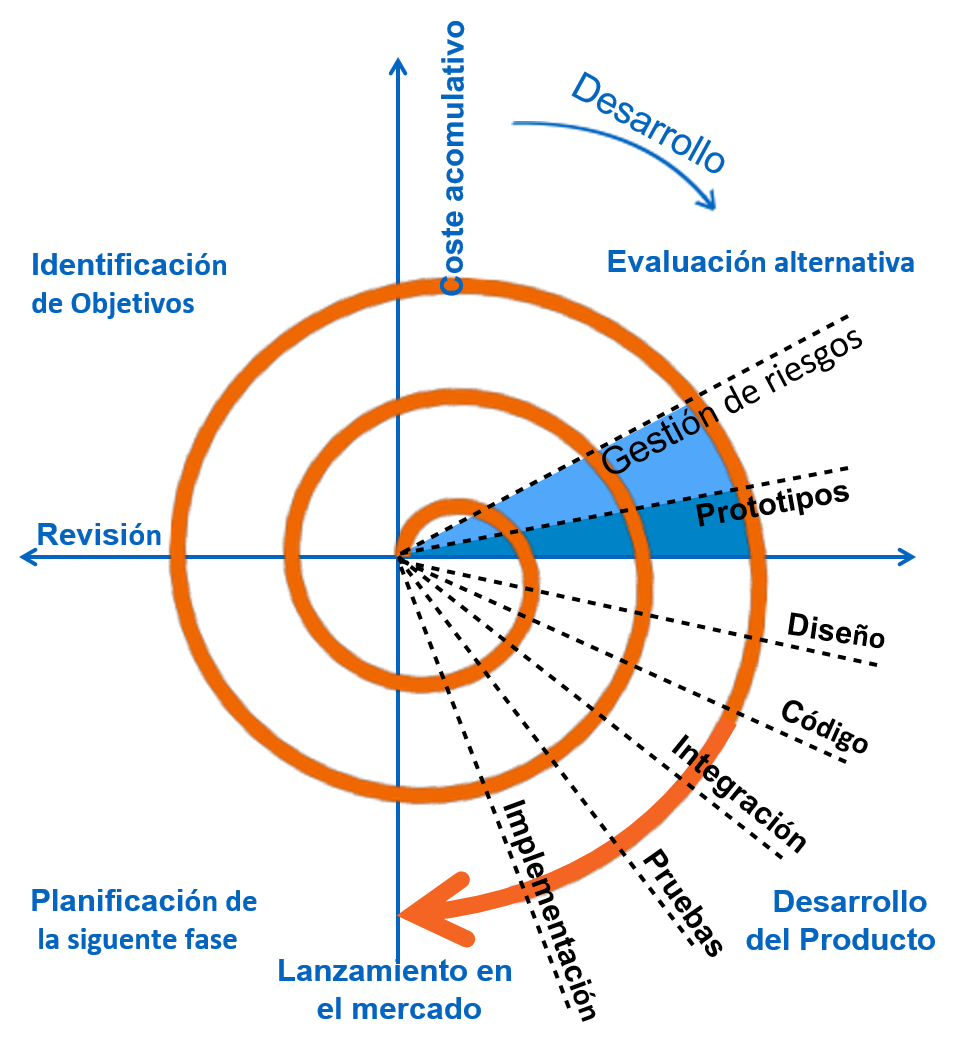
\includegraphics[scale=0.5]{espiral.jpg}
\caption{Modelo espiral del proceso de \textit{software} Boehm B. (1988).}
\end{figure}

Los nuevos requerimientos del sistema se definieron con todos los detalles posibles, esto implica generalmente el entrevistarse con un n\'umero determinado  de usuarios que representar\'an a todos los usuarios tanto externos como internos y otros aspectos del sistema existente. Un prototipo preliminar se cre\'o  para el desarrollo del nuevo \textit{software}  partiendo de un diseño hecho del sistema que se construy\'o del prototipo inicial. Esto es generalmente un sistema  scaled-down, y represent\'o una aproximaci\'on de las caracter\'isticas del producto final.\\
 
Este primer prototipo se desarrollo bajo las siguientes caracter\'isticas u objetivos de \textit{software} a alcanzar:  las funciones base para la carga de datos, los c\'alculos para el ajuste de modelos para los datos longitudinales y el desarrollo de los gr\'aficos se realizar\'ia bajo los paquetes que proporciona lenguaje R en su CRAN y en sus extensiones; la interfaz gr\'afica de usuario (GUI)  ser\'ia bajo un ambiente WEB simple y ligera, que se adaptara a la GUI del Laboratorio de Investigaciones Hormonales del IHULA, donde el gasto computacional fuera la estimaci\'on del modelo para datos longitudinales, esta se realizar\'ia en el lenguaje Java y se emplear\'ian el  paquete rJava para la conexi\'on lenguaje R y Java, adem\'as de JDK (\textit{Java SE Development Kit}) Eclipse. Durante esta etapa el an\'alisis de riesgo determin\'o que al desarrollar la GUI de usuarios bajo Java, seria necesario tener a la disposici\'on un servidor de forma permanente, lo que hace que la aplicaci\'on fuera poco portable. As\'i que se toma la desici\'on de cambiar el ambiente de desarrollo para la GUI.\\ 

Un segundo diseño de \textit{software} fue desarrollado por un procedimiento cu\'adruple: Evaluaci\'on del primer prototipo en t\'erminos de sus fuerzas, debilidades, y riesgos; Definir los requisitos del segundo prototipo; Planeando y desarrollando el segundo prototipo; Construyendo y probando el segundo prototipo. \\

El segundo diseño de \textit{software} mantuvo las caracter\'isticas seleccionadas para el primer diseño sobre el c\'alculos y las herramientas gr\'aficas pero la GUI se desarrolla empleando el paquete \textit{Shiny} del IDE RStudio, lo que permite tener un servidor local para cada usuario. \\

Adem\'as, se construy\'o el sistema final al que se denomin\'o HIVmlm (Human Immunology Virus linear model mixed effects), basado en el segundo diseño pero mejorando las caracter\'isticas de la GUI en la  Figura 3.3, se  muestra el\textit{wireframe} siguiendo el modelo basado en experiencia de usuario. El sistema final se eval\'uo y se probo con metodos de caja blanca y caja negra.\\


\begin{figure}[H]
\centering
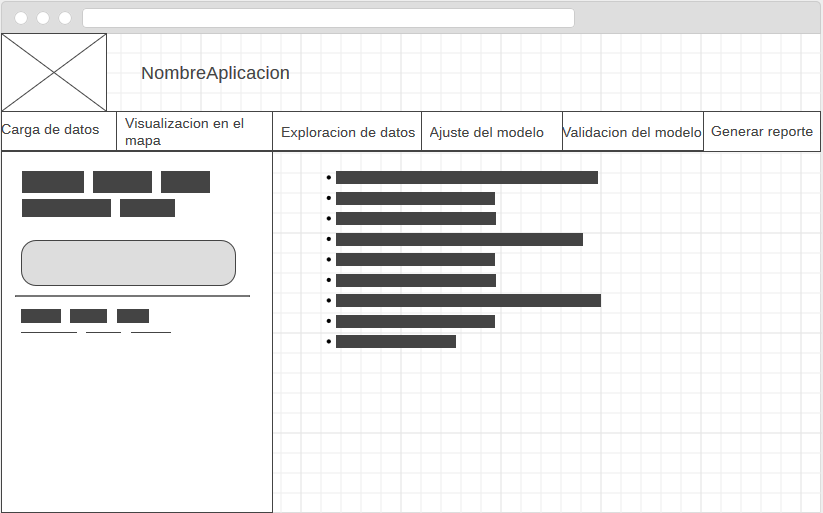
\includegraphics[scale=0.6]{etapa1_wireframe.png}
\caption{Wireframe base de la interfaz gr\'afica de usuario}
\end{figure}





